\documentclass[10pt,a4paper,openright]{report}

\usepackage[a4paper,top=0.82in,bottom=0.78in,left=0.78in,right=0.78in]{geometry}
\usepackage{amsmath,amssymb}
\usepackage{booktabs,tabularx,array,multirow,longtable}
\usepackage{graphicx}
\usepackage{enumitem}
\usepackage{microtype}
\usepackage{setspace}
\usepackage{titlesec}
\usepackage{fancyhdr}
\usepackage{caption}
\usepackage{subcaption}
\usepackage{hyperref}
\usepackage{float}
\usepackage{xcolor}
\usepackage{tikz}
\usetikzlibrary{arrows.meta,positioning}

\hypersetup{hidelinks}
\setstretch{1.04}
\setlength{\parindent}{0pt}
\setlength{\parskip}{4pt}
\setlist{leftmargin=1.5em,itemsep=2pt,topsep=3pt}
\setcounter{tocdepth}{1}
\setcounter{secnumdepth}{2}

\titleformat{\chapter}[display]
  {\normalfont\large\bfseries}
  {Chapter \thechapter}
  {1.2ex}
  {\Large\bfseries}
\titlespacing*{\chapter}{0pt}{22pt}{18pt}
\titleformat{\section}{\normalfont\normalsize\bfseries}{\thesection}{0.55em}{}
\titleformat{\subsection}{\normalfont\normalsize\bfseries}{\thesubsection}{0.5em}{}
\titlespacing*{\section}{0pt}{9pt}{4pt}
\titlespacing*{\subsection}{0pt}{7pt}{3pt}

\pagestyle{plain}
\fancyhf{}
\fancyfoot[C]{\thepage}
\renewcommand{\headrulewidth}{0pt}

\newcommand{\projecttitle}{Stackelberg-Based Adversarial Training for Robust EEG Classification}
\newcommand{\R}{\mathbb{R}}
\newcommand{\bacc}{\mathrm{bACC}}
\newcommand{\blankpage}{\clearpage\null\thispagestyle{plain}\clearpage}
\newcommand{\sg}{\operatorname{sg}}

\begin{document}
\setcounter{page}{1}

% -----------------------------------------------------------------------------
% PAGE 1: TITLE PAGE
% -----------------------------------------------------------------------------
\begin{titlepage}
\thispagestyle{empty}
\centering
\vspace*{0.1cm}
{\small\bfseries A REPORT\par}
\vspace{0.2cm}
{\small\bfseries ON\par}
\vspace{0.3cm}
{\large\bfseries \MakeUppercase{\projecttitle}\par}
\vspace{1.0cm}
{\small\bfseries BY\par}
\vspace{0.7cm}

\renewcommand{\arraystretch}{1.25}
\begin{tabular}{>{\raggedright\arraybackslash}p{0.31\textwidth}
                >{\centering\arraybackslash}p{0.22\textwidth}
                >{\raggedright\arraybackslash}p{0.35\textwidth}}
\textbf{Name of the student} & \textbf{ID No.} & \textbf{Discipline} \\
Pratham & F20240828 & B.E. Electronics and Communication Engineering
\end{tabular}

\vfill
Prepared in partial fulfillment of the requirements of the\\[0.1cm]
{\bfseries Practice School - I}
\vspace{0.55cm}

{\bfseries AT}\\[0.25cm]
{\large\bfseries FanPlay IOT}
\vspace{0.38cm}

A Practice School - I Station of
\vspace{0.15cm}

\includegraphics[width=2.05cm]{/mnt/data/assets/template-000.png}
\vspace{0.15cm}

{\small\bfseries BIRLA INSTITUTE OF TECHNOLOGY \& SCIENCE, PILANI}\par
\vspace{0.28cm}
July, 2026
\end{titlepage}
\setcounter{page}{2}

% -----------------------------------------------------------------------------
% PAGE 2: PROJECT INFORMATION
% -----------------------------------------------------------------------------
\thispagestyle{empty}
\begin{center}
{\small\bfseries BIRLA INSTITUTE OF TECHNOLOGY \& SCIENCE, PILANI}\\[-1pt]
{\small Practice School Division}
\end{center}
\vspace{0.2cm}

\small
\renewcommand{\arraystretch}{1.17}
\begin{tabularx}{\textwidth}{>{\bfseries}p{0.28\textwidth} X}
Station Centre & FanPlay IOT, FSID, IISc Incubator, Bengaluru \\
Duration & 25 May 2026 -- 22 June 2026 \\
Date of start & 25 May 2026 \\
Date of submission & 16 July 2026 \\
Title of the project & \projecttitle \\
ID No., name and discipline & F20240828, Pratham, B.E. Electronics and Communication Engineering \\
Name of the expert & Purnima Prashant \\
Name of the PS faculty member & Vinaya Kumar N \\
Key words & EEG, EEGNet, brain-computer interface, adversarial training, Stackelberg game, Euclidean alignment, PGD-CW, knowledge distillation \\
Project areas & Machine learning, biomedical signal processing, robust deep learning, EEG-based BCI classification \\
\end{tabularx}

\vspace{0.12cm}
\textbf{Abstract:}
This project studied how to make EEGNet classifiers more reliable when electroencephalography (EEG) signals contain small but harmful perturbations. The work began with a survey of EEG acquisition, channel selection, cognitive-state datasets and the difficulties caused by subject variability, artifacts and session drift. EEGMAT was selected as the main dataset because it provides resting-state and mental-arithmetic recordings from 36 subjects. The implementation evolved from preliminary sliding-window baselines to a compact EEGNet trained with Euclidean alignment, class balancing and adversarial objectives. The main proposed method models the classifier as the leader and the adversary as the follower in a Stackelberg game, allowing the leader update to account approximately for how the attack changes with the model parameters. Standard $\ell_\infty$ PGD, Carlini--Wagner margin attacks, and EEG-aware total-variation and power-spectral-density constraints were investigated. The supplied ablation results show that representative Stackelberg runs preserved or improved clean metrics relative to benign and plain-PGD baselines, although the benefit varied with alignment, attack constraints and random seed. The final notebook adds an eight-channel grouped leave-subject-out pipeline, causal Euclidean alignment, PGD-CW evaluation, knowledge distillation and TorchScript export. Since the notebook snapshot has no stored execution outputs, this report does not invent LOSO or deployment scores.

\vfill
\begin{tabularx}{\textwidth}{X X}
\textbf{Signature of the student} & \textbf{Signature of the PS faculty member} \\[0.75cm]
Date: 16 July 2026 & Date: 16 July 2026
\end{tabularx}
\normalsize
\clearpage

% -----------------------------------------------------------------------------
% PAGE 3: ACKNOWLEDGEMENTS
% -----------------------------------------------------------------------------
\chapter*{Acknowledgements}
\addcontentsline{toc}{chapter}{Acknowledgements}
\par\noindent
I would like to thank my PS faculty member, Vinaya Kumar N, for his guidance and feedback throughout the project. I am also grateful to my expert, Purnima Prashant, and to FanPlay IOT for giving me the opportunity to work on a research-oriented problem involving EEG signal processing, deep learning and adversarial robustness.

\par\noindent
I would also like to thank BITS Pilani and the Practice School Division for providing a structure in which I could connect theoretical ideas with implementation. During the project, I learned that an experimental machine-learning result is not only a model score. Fair comparison requires the same data split, preprocessing, optimizer, number of epochs, checkpoint rule, attack strength and random-seed policy. These lessons were especially important for EEG because subject variability and class imbalance can easily hide or exaggerate an improvement.

\vfill
\hfill\textbf{Signature of the student}
\clearpage

% PAGE 4
\null\thispagestyle{plain}\clearpage

% PAGE 5
\tableofcontents
\clearpage

% PAGE 6
\null\thispagestyle{plain}\clearpage

% PAGE 7
\listoffigures
\clearpage

% PAGE 8
\null\thispagestyle{plain}\clearpage

% PAGE 9
\listoftables
\clearpage

% PAGE 10
\null\thispagestyle{plain}\clearpage

% -----------------------------------------------------------------------------
% CHAPTER 1
% -----------------------------------------------------------------------------
\chapter{Introduction}

\section{Background}
Electroencephalography (EEG) records small voltage changes produced by the synchronized activity of groups of neurons. In a typical setup, metal electrodes are placed on the scalp using a standardized arrangement such as the International 10--20 system. A conductive medium reduces skin-electrode impedance, an amplifier strengthens the microvolt-level signal, and an analog-to-digital converter samples it at a fixed rate. Each channel therefore represents a voltage waveform measured at one scalp location relative to a reference electrode.

EEG is attractive for brain-computer interfaces because it is non-invasive, relatively inexpensive and has high temporal resolution. At the same time, the signal is weak and easily affected by eye blinks, muscle activity, electrode drift, external electrical interference and changes in mental state. Even recordings from the same person can change between sessions. A classifier may therefore memorize recording-specific noise instead of learning the neural pattern related to the task.

\begin{figure}[H]
\centering
\includegraphics[width=0.93\textwidth]{/mnt/data/assets/ps1p43/img-003.png}
\caption{Example of a multi-channel EEG recording from the EEGMAT data explored during the project.}
\label{fig:raw-eeg}
\end{figure}

\section{Problem statement}
Deep-learning models can classify EEG directly from the time domain, but they can also be sensitive to adversarial perturbations. Given a classifier $f_\theta$ and an input $x$, an attacker searches for a small $\delta$ such that $f_\theta(x+\delta)$ changes while $x+\delta$ remains close to the original signal. This is relevant even when there is no malicious attacker, because an adversarial example can be viewed as a worst-case model of small measurement changes.

The problem is more difficult in subject-independent BCI. Skull thickness, scalp conductivity, electrode placement and recording hardware produce large domain shifts across people. A model trained on one group may perform poorly on a new subject, and adversarial training can further reduce clean accuracy if it is not combined with an alignment strategy.

\section{Objectives and scope}
The main objectives of the project were:
\begin{enumerate}
\item to understand EEG acquisition, channel selection, preprocessing and dataset design;
\item to build an EEGNet baseline for resting-state versus mental-arithmetic classification on EEGMAT;
\item to study Euclidean alignment for reducing subject- and session-dependent covariance differences;
\item to compare an undefended EEGNet, plain PGD adversarial training and Stackelberg-style adversarial training;
\item to study $\ell_\infty$, total-variation and power-spectral-density constraints on the perturbation;
\item to design a grouped leave-subject-out, eight-channel and deployment-oriented extension with knowledge distillation.
\end{enumerate}

The project did not claim that a single adversarial-training run proves universal robustness. The supplied ablations were used to identify useful trends and experimental risks, while the final grouped-LOSO notebook was kept separate because it has not been executed in the uploaded snapshot.

% -----------------------------------------------------------------------------
% CHAPTER 2
% -----------------------------------------------------------------------------
\chapter{Literature Review}

\section{EEGNet and compact EEG architectures}
EEGNet is a compact convolutional neural network designed for EEG-based BCI tasks \cite{lawhern}. A temporal convolution first learns frequency-selective filters. A depthwise spatial convolution then learns channel combinations without creating the large parameter count of a regular two-dimensional convolution. Finally, a separable convolution combines depthwise temporal processing with a pointwise channel-mixing operation. This factorization is useful because EEG datasets are usually much smaller than image datasets.

The project initially considered spectrogram-based CNNs. A spectrogram is useful for visualizing spectral energy, but the transformation can reduce access to exact waveform polarity, phase and event timing. These quantities matter for event-related potentials and time-locked EEG patterns. For this reason, the final implementation used raw time-domain epochs and an EEG-specific architecture.

\begin{figure}[H]
\centering
\includegraphics[width=0.76\textwidth]{/mnt/data/assets/ps1p34/img-002.png}
\caption{EEGNet structure: temporal convolution, depthwise spatial filtering, separable convolution and classification.}
\label{fig:eegnet}
\end{figure}

\section{Adversarial training}
Projected Gradient Descent (PGD) approximately solves the inner maximization problem
\begin{equation}
\max_{\|\delta\|_\infty\leq\epsilon} \mathcal{L}(f_\theta(x+\delta),y),
\end{equation}
by taking repeated sign-gradient steps and projecting the perturbation back into the allowed $\ell_\infty$ ball \cite{madry}. The Carlini--Wagner (CW) margin attack uses the difference between the strongest incorrect logit and the true-class logit, directly encouraging a decision-boundary crossing \cite{cw}.

Plain adversarial training treats the generated perturbation as fixed when the classifier parameters are updated. A Stackelberg formulation makes the order of decisions explicit: the classifier is the leader and the adversary is the follower. The leader update can include an approximation to the derivative of the follower's response with respect to the model parameters \cite{gao}. The practical implementation used a short differentiable follower for the hypergradient and a stronger detached follower for the adversarial or consistency signal.

\section{Euclidean alignment and preprocessing}
Euclidean alignment (EA) whitens the mean spatial covariance of EEG trials \cite{hewu}. If $X_n\in\R^{C\times T}$ is an EEG epoch, the reference covariance is
\begin{equation}
\overline{R}=\frac{1}{N}\sum_{n=1}^{N}X_nX_n^\top,
\qquad
\widetilde{X}_n=\overline{R}^{-1/2}X_n.
\end{equation}
After alignment, the average covariance becomes close to the identity matrix. This reduces subject-specific scale and correlation differences and can make a shared classifier easier to learn. Alignment-based adversarial training has therefore been proposed as a way to improve both accuracy and robustness in EEG-based BCIs \cite{abat}.

The literature survey also showed that preprocessing is not automatically beneficial. Filtering, artifact correction, baseline correction and detrending can change what the classifier learns. Heavy preprocessing may remove noise, but it may also remove discriminative structure. During the project, kurtosis was explored as a diagnostic for heavy tails, but it was not used as a strict acceptance rule: non-Gaussian tails can contain genuine EEG information, and forcing all data to look Gaussian can reduce class separability.

\section{Dataset and channel survey}
The early project document compared datasets with different channel budgets. Low-channel datasets such as STEW are useful for consumer-grade workload monitoring, medium-channel datasets such as EEGMAT provide a practical research baseline, and high-density datasets such as EEGMMIDB or BCI Competition IV support more detailed motor-imagery studies. Table~\ref{tab:dataset-survey} summarizes the main datasets considered during the project.

\begin{table}[H]
\centering
\small
\caption{Datasets reviewed during the project.}
\label{tab:dataset-survey}
\begin{tabularx}{\textwidth}{p{0.24\textwidth}p{0.14\textwidth}X}
\toprule
Dataset & Channels & Main use in the project survey \\
\midrule
EEGMAT & 23 & Resting-state versus mental-arithmetic classification; selected for implementation because it has 36 subjects and simple EDF organization. \\
EEGMMIDB & 64 & Standard motor-imagery benchmark with many subjects and broad 10--10 coverage. \\
BCI Competition IV 2a & 22 EEG + 3 EOG & Four-class motor imagery and session-to-session transfer. \\
STEW & 14 & Low-channel cognitive workload and consumer-device experiments. \\
DEAP & 32 & Emotion, arousal and physiological-state classification. \\
Stress-resilience HCI dataset & 32 & Multimodal stress, work and recovery states. \\
\bottomrule
\end{tabularx}
\end{table}

The deployment-oriented version selected F3, F4, Fz, P3, P4, Pz, O1 and O2. Frontal channels capture executive control and workload-related activity, parietal channels capture visuospatial and information-processing activity, and occipital channels provide visual-attention information. This montage was chosen as a practical compromise between functional coverage and hardware cost.

\begin{figure}[H]
\centering
\includegraphics[width=0.72\textwidth]{/mnt/data/assets/ps1p27/img-002.png}
\caption{International 10--20 electrode locations and the frontal, parietal and occipital regions used in the eight-channel design.}
\label{fig:montage}
\end{figure}

% -----------------------------------------------------------------------------
% CHAPTER 3
% -----------------------------------------------------------------------------
\chapter{Methodology}

\section{EEGMAT preparation}
EEGMAT contains recordings from 36 healthy volunteers. For each subject, the file ending in \texttt{\_1.edf} is the resting recording and the file ending in \texttt{\_2.edf} is the mental-arithmetic recording \cite{zyma}. The source data is sampled at 500 Hz. The final notebook resamples it to 256 Hz and creates non-overlapping two-second epochs, resulting in $T=512$ samples per epoch.

The first experiments used sliding-window segmentation because the original number of long recordings was too small for direct neural-network training. A fixed-length window moves across each recording and each window becomes a labeled sample. The final notebook uses non-overlapping windows to avoid making adjacent samples excessively similar. Each channel in each epoch is standardized independently across time:
\begin{equation}
\widetilde{x}_{c,t}=\frac{x_{c,t}-\mu_c}{\max(\sigma_c,10^{-6})}.
\end{equation}
This normalization uses no other trial or subject statistics.

\section{Causal Euclidean alignment}
The final notebook fits an alignment matrix for each subject using the resting block only. If the resting epochs are $X_1,\ldots,X_N$, the whitening matrix is computed from their mean covariance and then applied unchanged to both the rest and task epochs. This is more realistic than allowing future task trials to contribute to their own preprocessing transform.

\section{Model architecture}
The teacher EEGNet uses $F_1=8$, depth multiplier $D=2$, $F_2=16$ and dropout 0.5. Its stages are:
\begin{enumerate}
\item a temporal convolution that learns frequency-selective kernels;
\item a depthwise convolution across channels that learns spatial filters;
\item an average-pooling and dropout stage;
\item a separable temporal convolution followed by pointwise channel mixing;
\item a linear classifier for the two output classes.
\end{enumerate}
For the eight-channel input, the teacher has 3,282 trainable parameters. The compact student uses $F_1=4$, $D=1$, $F_2=8$ and dropout 0.25, giving 1,442 parameters.

\section{Clean and plain-PGD training}
The clean model is trained using cross-entropy with label smoothing, Adam optimization, weight decay and cosine-annealed learning rate. Since the resting and task classes are imbalanced, a weighted random sampler is used for the training loader. Checkpoints are selected using validation balanced accuracy.

The plain adversarial-training baseline starts from the clean checkpoint. Training PGD uses random initialization in $[-\epsilon,\epsilon]$, 10 sign-gradient steps, step size 0.01, two restarts and $\epsilon=0.10$. Validation uses a stronger PGD-CW attack with 50 steps, step size 0.005 and five restarts.

\section{Stackelberg training}
The Stackelberg method represents the classifier as a leader and the perturbation generator as a follower. The representative leader objective used in the project can be written as
\begin{equation}
\mathcal{L}_{\mathrm{leader}}=
\mathcal{L}_{\mathrm{CE}}(f_\theta(x),y)
+\mathcal{L}_{\mathrm{CW}}(f_\theta(x+\widetilde{\delta}(\theta)),y)
+\lambda\left\|f_\theta(x)-\sg\left[f_\theta(x+\delta^*)\right]\right\|_2^2,
\end{equation}
where $\widetilde{\delta}(\theta)$ is a short differentiable follower and $\delta^*$ is a stronger detached attack. Differentiating through $\widetilde{\delta}(\theta)$ gives an approximate hypergradient that plain PGD training does not contain.

\section{EEG-aware perturbation constraints}
The basic threat model is
\begin{equation}
x^{\mathrm{adv}}=x+\delta, \qquad \|\delta\|_\infty\leq\epsilon.
\end{equation}
Two additional constraints were investigated:
\begin{align}
TV(\delta) &= \sum_{c,t}|\delta_{c,t+1}-\delta_{c,t}|\leq\tau,\\
D_{\mathrm{PSD}}(x,x+\delta) &\leq\kappa_{\mathrm{psd}}.
\end{align}
The total-variation constraint encourages temporal smoothness. The PSD constraint limits the change in the spectral profile. These guardrails make the perturbation more physiologically plausible, but they can also weaken the attacker by shrinking its feasible set. For that reason, final model comparisons should use a common strong evaluation attack.

\section{Grouped leave-subject-out evaluation}
The latest notebook shuffles all 36 subjects with seed 42 and divides them into six disjoint held-out groups. Each fold holds out six subjects for testing and four additional subjects for validation, so every subject is tested exactly once. Clean pretraining and PGD fine-tuning each run for 30 epochs. Final robust evaluation uses 50-step, five-restart PGD-CW at $\epsilon\in\{0.05,0.10,0.15\}$.

The metrics are ordinary accuracy, balanced accuracy, macro-F1 and Cohen's $\kappa$. For two classes,
\begin{equation}
\bacc=\frac{1}{2}\left(\frac{TP_0}{TP_0+FN_0}+\frac{TP_1}{TP_1+FN_1}\right).
\end{equation}
The notebook also computes a 95\% confidence interval across grouped folds and a paired Wilcoxon signed-rank test at $\epsilon=0.10$.

\section{Knowledge distillation and deployment}
The trained adversarial teacher can be distilled into the compact student using a weighted combination of hard-label cross-entropy and temperature-scaled KL divergence. The configured temperature is 4 and the soft-target weight is 0.7. Fold metadata, selected channels, alignment matrices and checkpoints are saved. The student can then be exported as a TorchScript file for deployment.

\begin{figure}[H]
\centering
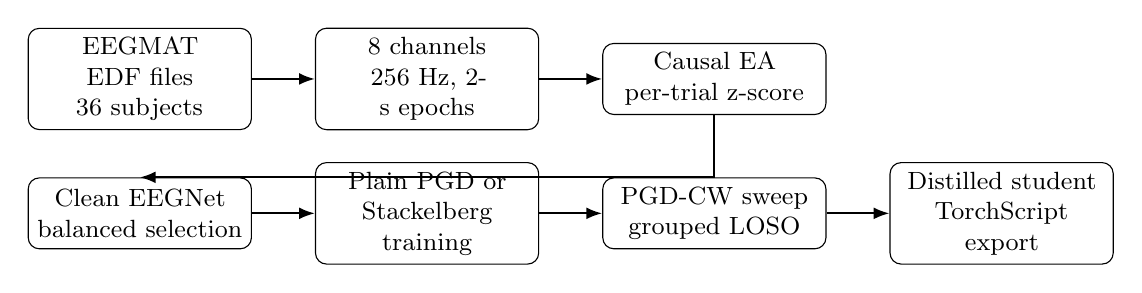
\begin{tikzpicture}[
node distance=6mm and 8mm,
box/.style={draw,rounded corners,align=center,minimum height=9mm,text width=2.6cm,font=\small},
arr/.style={-{Latex[length=2mm]},thick}
]
\node[box] (edf) {EEGMAT EDF files\\36 subjects};
\node[box,right=of edf] (prep) {8 channels\\256 Hz, 2-s epochs};
\node[box,right=of prep] (ea) {Causal EA\\per-trial z-score};
\node[box,below=of edf] (clean) {Clean EEGNet\\balanced selection};
\node[box,right=of clean] (adv) {Plain PGD or\\Stackelberg training};
\node[box,right=of adv] (eval) {PGD-CW sweep\\grouped LOSO};
\node[box,right=of eval] (kd) {Distilled student\\TorchScript export};
\draw[arr] (edf)--(prep);
\draw[arr] (prep)--(ea);
\draw[arr] (ea.south) |- (clean.north);
\draw[arr] (clean)--(adv);
\draw[arr] (adv)--(eval);
\draw[arr] (eval)--(kd);
\end{tikzpicture}
\caption{Final experimental and deployment pipeline represented by the supplied notebook.}
\label{fig:pipeline}
\end{figure}

% -----------------------------------------------------------------------------
% CHAPTER 4
% -----------------------------------------------------------------------------
\chapter{Results and Discussions}

\section{Preliminary baseline development}
The early implementation stage used sliding windows and a simpler training setup. One stored run reported an accuracy of approximately 73.23\%. The accompanying training and validation curves showed rapid convergence and a small but stable generalization gap. These experiments were useful for checking the EDF loader, labels, epoch extraction and basic EEGNet implementation before adding adversarial training.

\begin{figure}[H]
\centering
\begin{subfigure}[t]{0.48\textwidth}
\centering
\includegraphics[width=\textwidth]{/mnt/data/assets/ps1p46/img-002.png}
\caption{Training and validation loss.}
\end{subfigure}\hfill
\begin{subfigure}[t]{0.48\textwidth}
\centering
\includegraphics[width=\textwidth]{/mnt/data/assets/ps1p47/img-002.png}
\caption{Training and validation accuracy.}
\end{subfigure}
\caption{Preliminary EEGNet baseline curves from the PS-I project document.}
\label{fig:baseline-curves}
\end{figure}

A later vanilla EEGNet experiment in the supplied evaluation slides reached 82.54\% validation accuracy. In the matched ablation runs, the best benign validation accuracy was approximately 80.33--81.31\%, depending on the particular configuration and checkpoint rule. The difference between the early and later values illustrates why experimental settings must be recorded with the result.

\section{Clean test metrics}
Table~\ref{tab:clean-results} summarizes representative clean test metrics from the supplied ablation document. The rows come from separate reported configurations, so they should not be interpreted as one jointly randomized experiment.

\begin{table}[H]
\centering
\small
\caption{Representative clean test metrics from the supplied ablation results.}
\label{tab:clean-results}
\begin{tabular}{lcccc}
\toprule
Model/configuration & $A_{clean}$ & $\bacc_{clean}$ & F1 & $\kappa$ \\
\midrule
Clean EEGNet (baseline A) & 0.6869 & 0.6221 & 0.6127 & 0.2282 \\
Stackelberg $\ell_\infty$ & 0.7213 & 0.6388 & 0.6370 & 0.2741 \\
Clean EEGNet (baseline B) & 0.6984 & 0.6276 & 0.6207 & 0.2429 \\
Plain PGD $\ell_\infty$ & 0.6754 & 0.6208 & 0.6073 & 0.2200 \\
Plain PGD-CW + PSD + TV & 0.6721 & 0.6186 & 0.6047 & 0.2152 \\
Stackelberg $\ell_\infty$ + TV & 0.7213 & 0.6388 & 0.6370 & 0.2741 \\
Stackelberg $\ell_\infty$ + PSD + TV & 0.7213 & 0.6388 & 0.6370 & 0.2741 \\
\bottomrule
\end{tabular}
\end{table}

In the representative matched runs, plain adversarial training reduced all four clean metrics relative to baseline B. The Stackelberg $\ell_\infty$ run improved clean accuracy by 3.44 percentage points and balanced accuracy by 1.67 points over baseline A. This is consistent with the possibility that the leader-follower objective behaves like a useful regularizer. However, it is not enough to prove causality because training duration, checkpoint selection and seed must remain identical.

\section{Guardrail ablations}
The stored best validation robust balanced accuracies were 0.1178 for pure $\ell_\infty$ Stackelberg training, 0.1569 for $\ell_\infty$+TV and 0.1139 for $\ell_\infty$+PSD. The TV-constrained run had the largest stored validation value, but this does not automatically mean that it learned the strongest defense. A TV or PSD constraint reduces the attacker's freedom and may make the validation attack easier to resist.

The clean metrics also depended on the guardrail configuration. One PSD run improved clean accuracy from 0.6869 to 0.7148 and clean balanced accuracy from 0.6221 to 0.6365, while another PSD configuration produced only a small change. The correct interpretation is that EEG-aware constraints change both physiological plausibility and optimization difficulty. A common unconstrained or standardized evaluator is still required for fair comparison.

\section{Euclidean-alignment and seed ablations}
The no-alignment experiment was sensitive to the implementation details. With one changed-hyperparameter configuration, clean balanced accuracy increased from 0.6107 to 0.6363 under Stackelberg training. With the original hyperparameters it changed only from 0.5642 to 0.5648. This suggests that EA is helpful, but it also shows that the measured contribution of Stackelberg training depends on the full pipeline.

Seed sensitivity was also visible. For seed 7, the stored Stackelberg checkpoint had the same clean accuracy as the benign checkpoint (0.7230) but lower balanced accuracy (0.6101 instead of 0.6335). Therefore, the project does not claim that Stackelberg training improves every metric for every seed. Multiple seeds or subject-level repeated evaluation are required.

\section{Status of the grouped-LOSO extension}
The supplied eight-channel notebook is implementation-complete. It constructs six grouped held-out folds, trains clean and plain-PGD models, evaluates them using vectorized multi-restart PGD-CW, computes confidence intervals and a paired Wilcoxon test, saves causal-EA metadata and optionally distills a compact student. However, every output cell in the uploaded notebook is empty. Consequently, no grouped-LOSO, confidence-interval, Wilcoxon or distilled-student result is presented as a measured result in this report.

% -----------------------------------------------------------------------------
% CHAPTER 5
% -----------------------------------------------------------------------------
\chapter{Conclusions and Future Work}

The project produced a complete experimental framework for robust EEG classification. It covered EEG acquisition and dataset selection, raw-data inspection, sliding-window epoching, compact EEGNet design, Euclidean alignment, PGD and CW attacks, Stackelberg-style bilevel optimization, physiological guardrails, structural ablations and a deployment-oriented student model.

The available results indicate that representative Stackelberg runs can preserve better clean performance than plain PGD adversarial training and can improve robustness relative to an undefended EEGNet under some matched attacks. At the same time, the no-EA and seed ablations show that the gain is not universal. Guardrails can also make an attack more realistic while making it weaker, so robustness claims must always state the exact threat model.

The most important future step is to execute the final six-fold notebook and report fold-level mean, 95\% confidence interval and paired statistical tests for the clean EEGNet, plain PGD baseline, Stackelberg model and distilled student. The same held-out groups, alignment matrices, checkpoint rule and PGD-CW evaluator should be used for all models. After this, the study can be extended to BCI Competition IV, EEGMMIDB, ERP and workload datasets. A larger benchmark would show whether the method improves generalization beyond the specific rest-versus-arithmetic task.

Additional future work includes stronger attack validation, subject-wise channel selection learned only from training subjects, calibration of predictive confidence, and real-time inference tests on low-channel hardware. The eight-channel student should also be compared against the teacher in parameter count, latency, clean accuracy and robust accuracy.

% -----------------------------------------------------------------------------
% CHAPTER 6
% -----------------------------------------------------------------------------
\chapter{Recommendations}

\begin{enumerate}
\item Use exactly the same subject folds, Euclidean-alignment rule, optimizer, number of epochs, checkpoint criterion and evaluation attack for all model comparisons.
\item Report balanced accuracy, macro-F1 and Cohen's $\kappa$ in addition to ordinary accuracy because EEG datasets are often imbalanced.
\item Separate attack plausibility from attack strength. TV and PSD constraints may be useful during training, but every model should also be evaluated using one common strong $\ell_\infty$ attack.
\item Run multiple seeds or complete subject-wise folds and report uncertainty. A single favorable seed should not be used as the final result.
\item Keep test-subject data out of hyperparameter selection and alignment fitting. The causal rest-only EA design in the final notebook is a useful deployment-oriented choice.
\item Evaluate the distilled student under the same PGD-CW sweep as the teacher before making robustness claims about deployment.
\item Save subject splits, channel names, whitening matrices, normalization rules, attack hyperparameters and software versions with each checkpoint.
\item Extend the experiments to a standard motor-imagery benchmark and an ERP/workload benchmark to test whether the conclusions generalize across EEG paradigms.
\end{enumerate}

% -----------------------------------------------------------------------------
% BIBLIOGRAPHY
% -----------------------------------------------------------------------------
\cleardoublepage
\addcontentsline{toc}{chapter}{Bibliography}
\begin{thebibliography}{99}
\bibitem{lawhern}
V. J. Lawhern et al., ``EEGNet: A compact convolutional neural network for EEG-based brain-computer interfaces,'' \emph{Journal of Neural Engineering}, 2018.

\bibitem{zyma}
I. Zyma et al., ``Electroencephalograms during mental arithmetic task performance,'' \emph{Data}, 2019; dataset distributed through PhysioNet.

\bibitem{goldberger}
A. L. Goldberger et al., ``PhysioBank, PhysioToolkit, and PhysioNet: Components of a new research resource for complex physiologic signals,'' \emph{Circulation}, 2000.

\bibitem{madry}
A. Madry et al., ``Towards deep learning models resistant to adversarial attacks,'' \emph{International Conference on Learning Representations}, 2018.

\bibitem{cw}
N. Carlini and D. Wagner, ``Towards evaluating the robustness of neural networks,'' \emph{IEEE Symposium on Security and Privacy}, 2017.

\bibitem{gao}
R. Gao et al., ``Adversarial training and provable robustness: A Stackelberg game perspective,'' arXiv:2207.08137, 2022.

\bibitem{hewu}
H. He and D. Wu, ``Transfer learning for brain-computer interfaces: A Euclidean space data alignment approach,'' \emph{IEEE Transactions on Biomedical Engineering}, 2020.

\bibitem{abat}
X. Chen, Y. Wang and D. Wu, ``Alignment-based adversarial training for improving the robustness and accuracy of EEG-based BCIs,'' arXiv:2411.02094, 2024.

\bibitem{kessler}
Kessler et al., ``How EEG preprocessing shapes decoding performance,'' 2025.
\end{thebibliography}

% -----------------------------------------------------------------------------
% APPENDIX
% -----------------------------------------------------------------------------
\appendix
\chapter{Implementation Details}

\section{Main notebook settings}
\begin{table}[H]
\centering
\small
\caption{Main configuration of the grouped-LOSO notebook.}
\begin{tabularx}{\textwidth}{p{0.36\textwidth}X}
\toprule
Item & Setting \\
\midrule
Selected channels & F3, F4, Fz, P3, P4, Pz, O1, O2 \\
Target sampling rate & 256 Hz \\
Epoch length & 2 seconds (512 samples) \\
Grouped folds & 6 folds, 6 test subjects per fold \\
Validation subjects & 4 subjects per fold \\
Clean training & 30 epochs, Adam, cosine annealing \\
Adversarial training & 30 epochs, $\epsilon=0.10$, 10 PGD steps, step size 0.01, 2 restarts \\
Validation attack & PGD-CW, 50 steps, step size 0.005, 5 restarts \\
Evaluation budgets & $\epsilon=0.05,0.10,0.15$ \\
Teacher architecture & $F_1=8$, $D=2$, $F_2=16$, dropout 0.5 \\
Student architecture & $F_1=4$, $D=1$, $F_2=8$, dropout 0.25 \\
Distillation & Temperature 4, soft-target weight 0.7, 20 epochs \\
Deployment export & PyTorch checkpoint and TorchScript \\
\bottomrule
\end{tabularx}
\end{table}

\section{Reproducibility note}
The notebook stores the selected-channel metadata, fold split, per-subject causal-EA whitening matrices, model configuration and evaluation metrics with the checkpoint. This is important because a model file alone is not sufficient to reproduce an EEG experiment. The same preprocessing and alignment transform must be available during evaluation and deployment.

\end{document}
